% ==========================================================
% レポート(A4・3ページ版):イオントラップ量子コンピュータにおけるランダム測定
%   対象論文: T. Brydges et al., Science 364, 260 (2019).
%   コンパイル: lualatex iontrap_report.tex  (参照のため2回)
% ==========================================================
\documentclass[10pt,a4paper,twocolumn]{ltjsarticle}
\usepackage[haranoaji]{luatexja-preset}
\usepackage{amsmath,amssymb,bm}
\usepackage{graphicx}
\usepackage[margin=14mm]{geometry}
\usepackage[hidelinks]{hyperref}
\usepackage{xcolor}

\setlength{\columnsep}{6mm}
\setlength{\parindent}{1em}
\allowdisplaybreaks
\newcommand{\ev}[1]{\langle #1\rangle}
\newcommand{\ket}[1]{|#1\rangle}
\newcommand{\bra}[1]{\langle #1|}
\newcommand{\Tr}{\operatorname{Tr}}
\renewcommand{\baselinestretch}{1.0}

% セクション見出しを詰める
\usepackage{titlesec}
\titlespacing*{\section}{0pt}{4pt}{2pt}
\titleformat{\section}{\normalfont\bfseries\large}{\thesection}{0.5em}{}

\begin{document}

\twocolumn[{%
\begin{center}
{\LARGE\bfseries レポート:イオントラップ量子シミュレータにおける\\[2pt]
ランダム測定によるエンタングルメント測定}\\[6pt]
{\large 自分の研究(CRM シャドウによるハバード模型の測定効率化)との関連を中心に}\\[10pt]
{\normalsize 学籍番号:24B25028\qquad 名前:龍山 昊平}
\end{center}
\vspace{4pt}
\begin{center}
\begin{minipage}{0.92\textwidth}
\small
\textbf{対象論文:} T.~Brydges, A.~Elben, P.~Jurcevic, B.~Vermersch, C.~Maier, B.~P.~Lanyon,
P.~Zoller, R.~Blatt, C.~F.~Roos, ``Probing R\'enyi entanglement entropy via randomized measurements'',
\textit{Science} \textbf{364}, 260--263 (2019) [arXiv:1806.05747].\par
\smallskip
\textbf{要旨:} イオントラップの量子シミュレータの上でランダム測定を使い、エンタングルメント
エントロピーを測ったのがこの論文である。これを選んだのは、自分がいま取り組んでいる研究、
つまり共通ランダム測定シャドウ(CRM シャドウ)でハバード模型の測定を効率化するという研究が、
この論文で実証されている「ランダムな局所ユニタリを掛けてから射影測定する」というやり方を
そのまま土台にしているからである。しかも著者の Vermersch と Elben は、自分の研究の出発点になった
CRM の原論文の著者でもある。このレポートでは、まず論文の内容をまとめ、そのうえで自分がこれまでの
数値計算で得た結果と論文の中身がどこでつながっているのかを整理してみる。
\end{minipage}
\end{center}
\vspace{10pt}
}]

% =====================================================================
\section{はじめに:自分の研究とこの論文}
% =====================================================================
最初に、話の前提として自分がやっていることを簡単に書いておく。量子コンピュータや量子シミュレータの
中にできた状態 $\rho$ について、物理量の期待値 $\ev{O}=\Tr[O\rho]$ を知りたいとする。量子測定は
結果が確率的にしか出ないので、精度を上げようとすると測定回数がすぐ膨大になる。これを減らすための
方法が古典シャドウ(ランダム測定)で、各量子ビットにランダムな基底を選んで射影測定し、その結果から
たくさんの物理量をまとめて推定する。さらにそれを改良したのが CRM シャドウ\cite{crm}である。考え方は
単純で、実験でできる状態 $\rho$ のだいたいの近似 $\sigma$(prior と呼ぶ)を古典計算で用意しておき、
実験に使ったのと\textbf{同じ乱数}を $\sigma$ にも当てて、
\begin{equation}
\hat o_{\rm CRM}=\overline{X_\rho(u)-X_\sigma(u)}+\Tr[O\sigma]
\label{eq:crm}
\end{equation}
のように差だけを統計的に推定する。あらかじめ分かっているぶんを引いてしまうので、ばらつきが減って
必要な測定回数が減る、というわけである。自分の研究は、この CRM を電子系の代表的な模型であるハバード
模型に合うように作り替え、prior をどう作れば得をするのかを数値計算で調べるものである。

この「ランダムな局所ユニタリを掛けてから射影測定を繰り返す」というやり方を、実際の装置で初めて
きちんとやってみせたのが Brydges たちのこの論文\cite{brydges}だった。著者を見ると Vermersch と Elben が
いて、この二人は自分が出発点にした CRM の原論文の著者でもある。つまり、Brydges の実証があって、
そこから古典シャドウ\cite{shadow}や CRM が出て、その先に自分のフェルミオン向けの CRM がある、という
流れになっている。だからこの論文は自分の研究のちょうど土台にあたると思って選んだ。

% =====================================================================
\section{イオントラップの基礎}
% =====================================================================
ランダム測定を実際の装置でやるには、少なくとも三つのことがいる。各量子ビットを別々に、しかも
精度よく回せること。一つ一つの量子ビットを個別に測れること。そのあいだ状態が十分に保たれる
(コヒーレンスが長い)こと。イオントラップはこのどれもかなり得意なので、実証の舞台に選ばれたの
だと思う。この論文では ${}^{40}\mathrm{Ca}^{+}$ イオンを線形 Paul トラップに一列に並べ、各イオンの
光学遷移($S_{1/2}$ と $D_{5/2}$)に量子ビットを乗せている。細く絞ったレーザーを当てて任意の回転
$R_z(\theta_3)R_y(\theta_2)R_z(\theta_1)$ をかけ、角度を乱数にすればランダムな局所ユニタリになる。
測定は、状態によって光り方が変わる蛍光を CCD で撮って一つずつ読み出す。イオンどうしは共通の
振動モードを通じて全対全でつながることができ、$J_{ij}\approx J_0/|i-j|^\alpha$ のような長距離の
相互作用も作れる。自分が計算のなかで置いている測定モデル、つまり各量子ビットごとにランダムな
基底を選んで射影測定するというやり方は、要するにこの装置でできることをそのまま抽象化したものだった。

% =====================================================================
\section{論文の内容}
% =====================================================================
\textbf{何をしたいか.} 部分系 $A$ の 2 次 R\'enyi エントロピー $S^{(2)}(\rho_A)=-\log_2\Tr[\rho_A^2]$ を
測りたい、というのがこの論文の目的である。純度 $\Tr[\rho_A^2]$ は密度行列について 2 次(非線形)の
量なので、素朴にやろうとすると同じ状態のコピーを 2 つ用意して同時に測る必要があった。この論文の
うまいところは、状態を一度に 1 つしか使わず、あとは古典計算の後処理だけで純度を出せる点である。

\textbf{やり方.} まず N\'eel 状態 $\ket{\downarrow\uparrow\cdots}$ を用意して、横磁場つきの長距離 XY 模型
$H=\hbar\sum_{i<j}J_{ij}(\sigma_i^+\sigma_j^-+\sigma_i^-\sigma_j^+)+\hbar B\sum_j\sigma_j^z$ で時間発展させる。
そのあと各量子ビットに CUE(1 量子ビットの Haar 分布)から引いた $u_i$ をかけ、$z$ 基底で射影測定する。
これを 1 設定あたり $N_M$ ショット、設定を $N_U$ 通り取り替えながら繰り返す。純度は、測定確率
$P(s)=\bra{s}U\rho U^\dagger\ket{s}$ の、違うビット列どうしの相関をアンサンブル平均することで復元できる。
\begin{equation}
X=2^{N_A}\!\!\sum_{s,s'}(-2)^{-D[s,s']}P(s)\,P(s'),\quad \Tr[\rho_A^2]=\overline{X}
\label{eq:est}
\end{equation}
ここで $D$ はハミング距離である。ざっくり言うと、純度は「ランダムに回したあとの測定結果のばらつき、
つまり分布の広がり」に化けている、というのが直感的な理解だと思う。

\textbf{結果.} 10 量子ビットの系を $N_U{=}500$、$N_M{=}150$ で測ると、全系の純度は
$\Tr[\rho^2]{=}0.74\pm0.07$ で、時間発展のあいだほぼ一定だった。これは発展がだいたいユニタリに
保たれている証拠になる。しかも 1 回とったデータから $2^{10}{-}1{=}1023$ 通りの分割すべての純度を
計算し直せて、$511$ 通りの二分割でエンタングルメントを確認している。20 量子ビットでは中央
10 量子ビットぶんのエントロピーが増えていく様子を測り、MPS の数値計算とよく合っていた。乱れを
入れると、エントロピーの増え方が鈍る、初期状態を覚えている、相互情報量が距離とともに減る、といった
多体局在らしい兆候も見えている。気になったのは系統誤差の話で、純度は状態準備で $0.08$、ランダムに
回している最中のデコヒーレンスで約 $0.17$ も小さめに出てしまう、とちゃんと見積もられていた。

\textbf{読んで思った要点.} 一つ目は、非線形でグローバルな量を、状態 1 コピーの測定と古典後処理だけで
測れること。二つ目は、そのかわり統計誤差が部分系サイズ $N_A$ とともに指数的に増えてしまうこと。
式\eqref{eq:est}の $2^{N_A}$ や、Fig.~2 でエラーバーが $N_A$ とともに広がっていくのがそれである\cite{toolbox_pra}。
三つ目は、ランダムに回す操作そのものの不完全さが、無視できない系統誤差になること。この三つは、
あとで自分の研究とつなげるときに効いてくる。

% =====================================================================
\section{自分の研究との関連}
% =====================================================================
ここが一番書きたかったところである。自分がこれまでの数値計算で得た結果と、この論文の内容とを、
思いついた順に 7 つの接点として並べてみる。

\textbf{(1) 測定のやり方がそもそも同じ.} 自分の CRM は、各量子ビットにランダムな基底($X/Y/Z$)を
選んで射影測定する、というのを $n_u$ 設定 $\times$ $n_m$ ショットぶん集めたデータの上に成り立っている。
これは本論文($N_U$ が $n_u$、$N_M$ が $n_m$ にあたる)とまったく同じ骨組みである。違うのは回す集団
だけで、Brydges は連続的な CUE(Haar)、自分は離散的なランダム Pauli を使っている。推定の式も
どちらも「測定というチャネルを逆に解く」ことから出てきていて、自分の式に出てくる係数 $3^{|A|}$
($|A|$ は観測量が乗っている量子ビットの数)は、本論文の式\eqref{eq:est}の $2^{N_A}(-2)^{-D}$ と
根っこが同じである。だから自分の CRM は、この論文でとった実験データにそのまま後処理としてかけられる、
という関係になっている。

\textbf{(2) 指数的な壁があるから局所量に逃げる.} 本論文の純度やエントロピーは非線形でグローバルな量
なので、誤差が $N_A$ とともに指数的に増える。じつはこれは自分がぶつかった壁とまったく同じだった。
自分の場合、prior が実験状態をどれくらい当てているかを測る指標として忠実度 $F$ を使っていたのだが、
これも状態について 2 次の量で、$L{=}32$ の鎖だと $F{=}0.007$ まで指数的に落ちてしまい、ランダム Pauli 測定
から忠実度を推定しようとすると指数的に破綻してしまう。そこで自分は、グローバルな量ではなく局所観測量、
つまり数サイトにしか乗っていない量のほうに的をしぼった。すると局所 Pauli 観測量 $P$ に対する CRM の
利得(分散が何倍減るか)は
\begin{equation}
G=\frac{(3^{|A|}-1)\ev{P}^2+v_s}{(3^{|A|}-1)\Delta^2+v_s},\quad \Delta\equiv\ev{P}_\rho-\ev{P}_\sigma
\label{eq:gain}
\end{equation}
という閉じた形になった($v_s$ はショットノイズの寄与)。ここで大事なのは、利得を決めるのが状態全体の
忠実度ではなく、その観測量についての prior のずれ $\Delta$ だけだという点である。おかげで、$F$ が
指数的に崩れても局所観測量の利得は鎖の長さ $L$ によらず生き残り、実際 $G$ はだいたい 12 から 57 だった。
要するに、本論文が「ここが一番高くつく」と示した領域を、自分は「そこは測らないで局所観測量に集中する」
ことでよけている、という関係になっていると思う。

\begin{figure}[t]
\centering
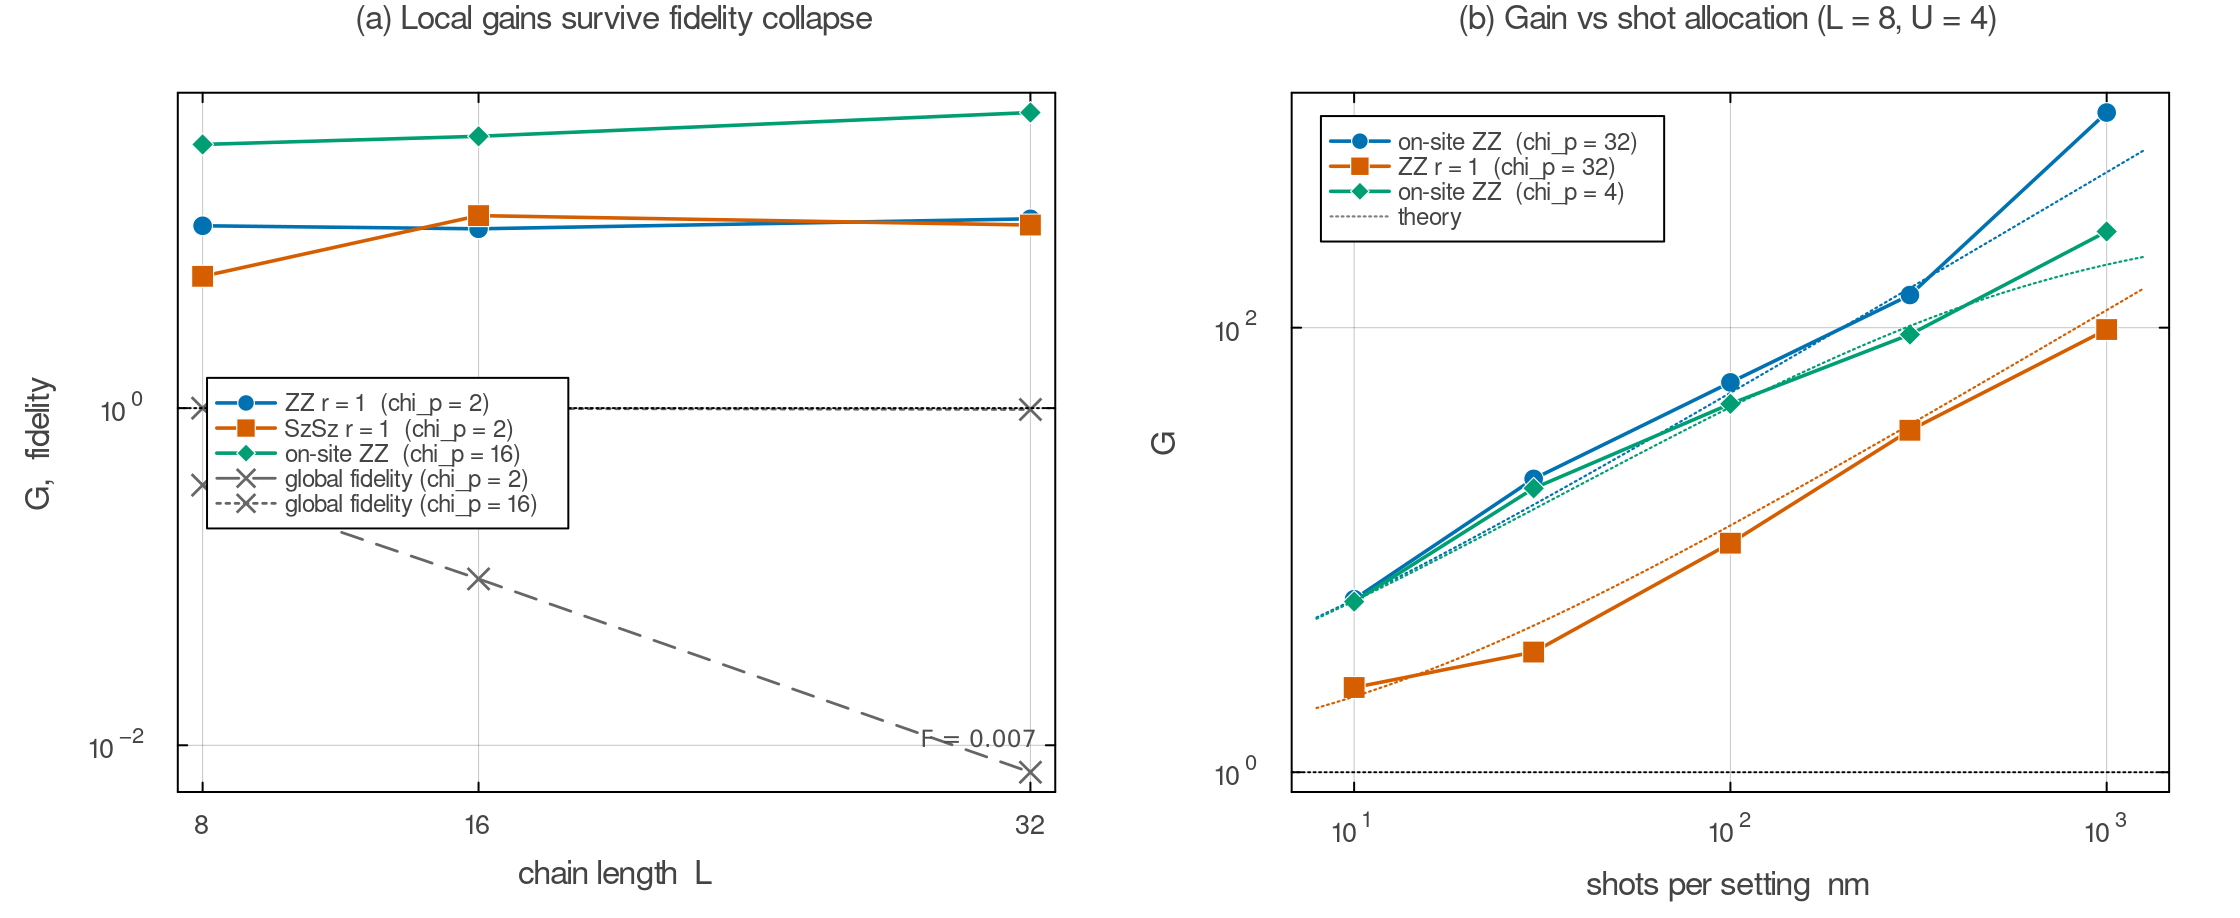
\includegraphics[width=\linewidth]{crm_fig2_locality.png}
\caption{\small 自分の数値計算から。1 次元ハバード鎖($U{=}4$)では、prior の忠実度 $F$ は
鎖の長さ $L$ とともに指数的に落ちる($L{=}32$ で $F{=}0.007$)のに、局所観測量の CRM 利得 $G$ は
$L$ によらず残っている。Brydges の実験で部分系サイズ $N_A$ とともにエントロピーの誤差が
増えていくのと、ちょうど裏表の関係になっている。}
\label{fig:loc}
\end{figure}

\textbf{(3) CRM はこの流れの直接の子ども.} 式\eqref{eq:crm}のように、CRM は prior $\sigma$ に同じ乱数 $u$ を
古典計算でかけて差をとることで分散を減らす手法である。自分がやったのはこれをフェルミオン向けに作り替える
ことで、具体的には次の三つを数値で確かめた。一つ目は、$O(N^3)$ の手間で作れる平均場(UHF)の prior が、
2 次元でも結合次元 $\chi{=}32$--$64$ の行列積状態(MPS)の prior に張り合えること。MPS は 2 次元だと
すぐ苦しくなるので、これは実用上ありがたい。二つ目は、prior は式\eqref{eq:crm}に期待値としてしか入らないので
混合状態でもよく、しかも古典後処理なので観測量ごとに別の prior を選んでよいこと。三つ目は、差の項に係数
$\beta$ を付けて同じデータから決めてしまえば、prior がよほど悪くても損をしないこと。どれも、測定は増やさずに
$N_U\times N_M$ を減らす方向の話である。

\textbf{(4) 測定の配分が目的で逆になる.} 純度のような非線形量は、分散が主に設定(ユニタリ)ごとの
ばらつきで決まるので、設定数を多くとるほうが得で、実際この論文でも $N_U{=}500$ と多い。ところが CRM だと、
設定ごとのゆらぎのほうが打ち消されて、残ったショットノイズを減らすことが効くので、設定を減らしてショットを
厚くするほうが得になる。同じ装置の同じようなデータでも、何を測りたいかで最適なつまみが逆向きになるのは
面白いと思った。

\textbf{(5) 同じデータを使い回す.} 本論文は 1 回のデータから 1023 通りの分割を全部計算し直していた。
どの分割にするかは古典後処理で決めている。これは自分がやっている「同じデータに対して、観測量ごとに
いちばん合う prior をあとから選ぶ」という発想とそっくりである。自分はさらに、複数の prior を回帰で
混ぜることで、平均場だけで作ったタダの prior でも $\chi{=}32$ の MPS prior くらいの利得まで届かせている。

\textbf{(6) フェルミオンと JW 弦、matchgate.} 本論文の装置が直接作れるのはスピン模型である。自分が扱うのは
電子(フェルミオン)なので Jordan--Wigner 変換でスピンに移すのだが、この変換はフェルミオンの反交換の符号を
非局所な「弦」として引きずってしまう。実際に 2 次元の系で計算してみると、横向きのホッピングの演算子が
9 量子ビットぶんに伸びてしまい、ランダム Pauli 測定ではほとんど測れなくなった。これを解くのが matchgate
(フェルミオンの Gauss)シャドウで、測定前にかける回転を Pauli ではなくフェルミオンの Gauss ユニタリにすると、
演算子の広がりによらず測れるようになり弦の問題が消える。自分の計算ではエネルギーの誤差が約 13 分の 1 になった。
matchgate に必要な非局所なゲートはイオンの全対全結合と相性がよいので、自分の手法を実機でやるならイオンは
有力な候補だと思う。ただし CRM の利得のほうは測定に使う集団しだいで、自己平均してしまう Gauss 回転だと
小さくなってしまうことも分かった。

\textbf{(7) デコヒーレンスと共通乱数.} 本論文の $0.17$ の過小評価は、回している最中のデコヒーレンスから
来ていた。CRM は同じ乱数 $u$ を $\rho$ と prior $\sigma$ の両方にかけて差をとる「共通乱数」の考え方なので、
ゆらぎだけでなく、共通して乗るような系統誤差もある程度は相殺できるかもしれない。ここから、実機のノイズを
prior 側にも取り込んでしまう robust な CRM\cite{robust} が次にやってみたい方向として見えてくる。正直に言うと、
いまの自分の実装は prior 側を理想的な $u$ で厳密に計算しているので、この相殺はまだできていない。

% =====================================================================
\section{さらに調べたこと・考えたこと}
% =====================================================================
\textbf{大きい系に向けて.} 同じ Innsbruck のグループは、このランダム測定を 51 イオンまで広げていて、
XXZ 鎖で最大 20 サイトの部分系についてエンタングルメント・ハミルトニアン(局所的な構造をもつ演算子)を、
少ない測定で学習している\cite{joshi}。さらに 2 次元で数百イオンという装置も出てきている\cite{2dions}。この
50 から数百量子ビットあたりが、じつは自分の研究がいちばん役に立ってほしい範囲である。この規模になると
忠実度も純度も測れないし、2 次元だと MPS の prior もすぐ崩れるので、$O(N^3)$ で作れる平均場の prior や、
観測量ごとに prior を選ぶ、係数 $\beta$ をデータから決めるといった「測定を増やさずに済ませる工夫」が
効いてくるはずだと考えている。

\textbf{考えたこと.} まず、自分の研究の意味は、Brydges がいちばん苦しんでいた領域を正面から突破することでは
なくて、局所観測量に逃げてそこを避けるところにあるのだと思う。両方は競争ではなく、グローバルな構造を
知りたいのか、局所的な物理量を知りたいのかで使い分けるものだと整理できた。つぎに、実験する人へ具体的に
言えることもある。占有やスピン相関、ホッピングのような局所量をねらうなら、「設定を多く・ショットは中くらい」
より「設定を減らしてショットを厚く、そこに CRM」のほうが得で、しかも装置を変えなくていい。あとは、共通乱数で
誤差を消すという CRM の性質を robust shadow のノイズ較正とつなげて、prior 側に実機ノイズを入れていくのが
次の課題だと感じた。最後に正直な限界として、自分の結果はどれも「固定した参照状態 $\rho$ に対する分散」の話で、
prior 側は理想的な測定を仮定してしまっている。Brydges がていねいに見積もっていた実機の粗さ、つまり準備の誤差や
回している最中のデコヒーレンス、コヒーレンス時間の限界をちゃんと取り込んで実データで確かめることが、自分の
手法を「計算のなかで分散が減る」から「実機で本当に測定回数が減る」へ進めるための次の一歩になると思う。

% =====================================================================
{\footnotesize
\begin{thebibliography}{9}
\setlength{\itemsep}{0pt}
\bibitem{brydges} T.~Brydges \textit{et al.}, ``Probing R\'enyi entanglement entropy via randomized measurements'',
\textit{Science} \textbf{364}, 260 (2019); arXiv:1806.05747.
\bibitem{crm} B.~Vermersch, A.~Rath, B.~Sundar, C.~Branciard, J.~Preskill, A.~Elben,
``Enhanced estimation of quantum observables with common randomized measurements'', \textit{PRX Quantum} \textbf{5}, 010352 (2024).
\bibitem{shadow} H.-Y.~Huang, R.~Kueng, J.~Preskill, \textit{Nat.~Phys.} \textbf{16}, 1050 (2020).(古典シャドウ)
\bibitem{toolbox_pra} A.~Elben, B.~Vermersch, C.~F.~Roos, P.~Zoller, \textit{Phys.~Rev.~A} \textbf{99}, 052323 (2019).
\bibitem{joshi} M.~K.~Joshi \textit{et al.}, ``Exploring large-scale entanglement in quantum simulation'',
\textit{Nature} \textbf{624}, 539 (2023); arXiv:2306.00057.(51 イオン)
\bibitem{2dions} S.-A.~Guo \textit{et al.}, ``A site-resolved two-dimensional quantum simulator with hundreds of trapped ions'',
\textit{Nature} \textbf{630}, 613 (2024).
\bibitem{robust} S.~Chen, W.~Yu, P.~Zeng, S.~T.~Flammia, ``Robust shadow estimation'', \textit{PRX Quantum} \textbf{2}, 030348 (2021).
\end{thebibliography}
}

\end{document}
